%%%%%%%%%%%%%%%%%%%%%%%%%%%%%%%%%%%%%%%%%
% Friggeri Resume/CV
% XeLaTeX Template
% Version 1.2 (3/5/15)
%
% This template has been downloaded from:
% http://www.LaTeXTemplates.com
%
% Original author:
% Adrien Friggeri (adrien@friggeri.net)
% https://github.com/afriggeri/CV
%
% License:
% CC BY-NC-SA 3.0 (http://creativecommons.org/licenses/by-nc-sa/3.0/)
%
% Important notes:
% This template needs to be compiled with XeLaTeX and the bibliography, if used,
% needs to be compiled with biber rather than bibtex.
%
%%%%%%%%%%%%%%%%%%%%%%%%%%%%%%%%%%%%%%%%%

\documentclass[]{friggeri-cv} % Add 'print' as an option into the square bracket to remove colors from this template for printing

\addbibresource{gkiarcv.bib} % Specify the bibliography file to include publications

\begin{document}

\header{gregory}{kiar}{biomedical engineer} % Your name and current job title/field

%----------------------------------------------------------------------------------------
%	SIDEBAR SECTION
%----------------------------------------------------------------------------------------

\begin{aside} % In the aside, each new line forces a line break
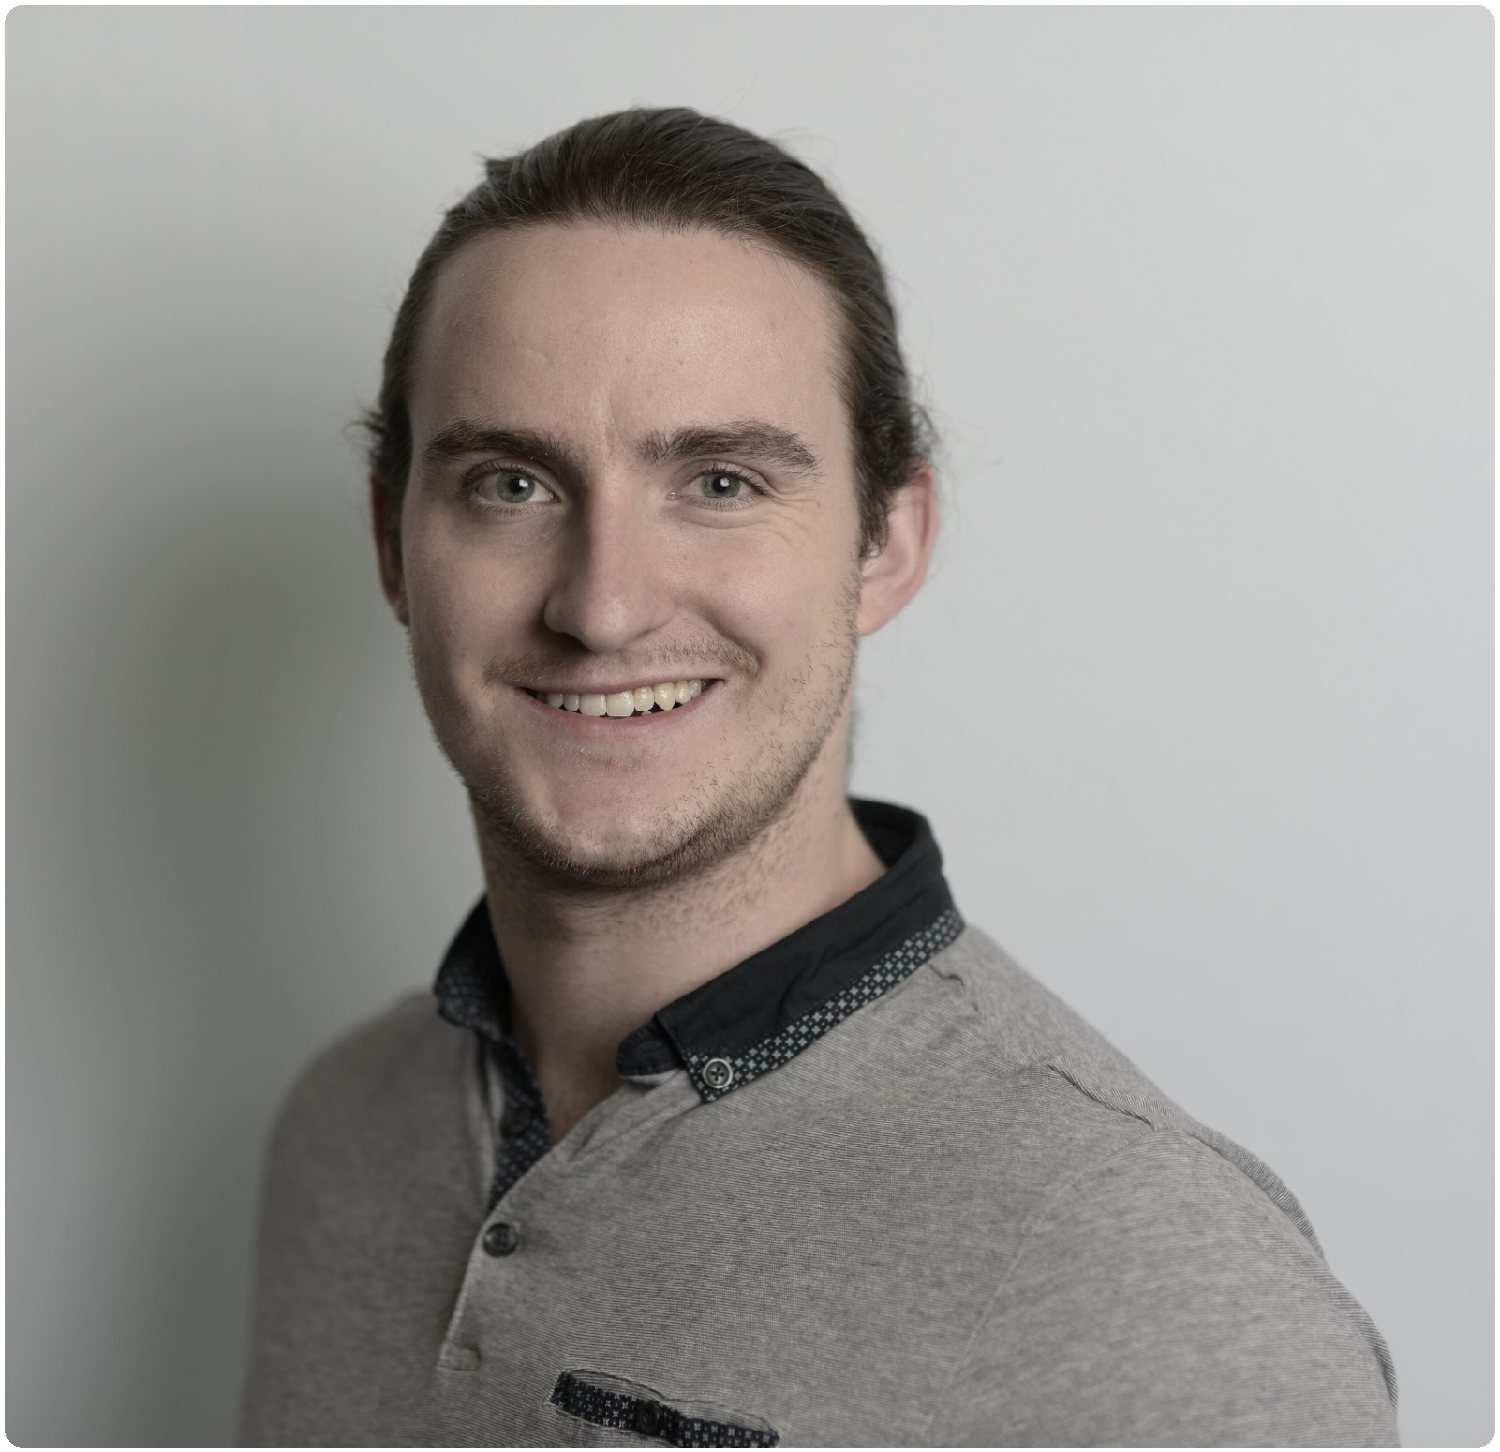
\includegraphics[width=\textwidth]{./headshot.pdf}
\section{contact}
2723 Saint Paul Street
Apartment 2
Baltimore, Maryland
21218, USA
~
+1 (443) 554 6865~{\color{green} \faMobilePhone}
+1 (443) 347 3455~{\color{green} \faMobilePhone}
~
\href{mailto:gkiar07@gmail.com}{gkiar07@gmail.com~{\color{red} \faEnvelope}}
\href{http://gkiar.github.io}{gkiar.github.io~{\color{brown} \faGlobe}}
\href{http://github.com/gkiar}{gkiar~{\color{purple} \faGithub}}
\href{https://www.linkedin.com/in/gregkiar}{gregkiar~{\color{blue} \faLinkedin}}
\section{languages}
english native speaker,
basic ASL
\section{programming}
Python, R, AWS {\color{red} $\varheartsuit$}
MATLAB, C++, x86,
LaTeX, CSS \& HTML
\section{soft skills}
leadership, design, problem~solving, teaching
\end{aside}

%----------------------------------------------------------------------------------------
%	EDUCATION SECTION
%----------------------------------------------------------------------------------------

\section{education}

\begin{entrylist}

%------------------------------------------------

\entry
{2014 -- 2016}
{M.S.E {\normalfont in Biomedical Engineering}}
{Johns Hopkins University, Baltimore, MD}
{Thesis work was supervised by Joshua T. Vogelstein on a project entitled:\\GREMLIN:
Graph Estimation from MR images Leading to Inference in Neuroscience.}

%------------------------------------------------

\entry
{2010 -- 2014}
{B.Eng {\normalfont in Biomedical and Electrical Engineering}}
{Carleton University, Ottawa, ON}
{Capstone work was supervised by Leonard MacEachern on a project entitled:\\Electrical
muscle stimulation with concurrent EMG feedback of the upper arm for applications in stroke
rehabilitation.}

%------------------------------------------------

\entry
{2016}
{Exploring the Human Connectome}
{The Human Connectome Project, Boston, MA}
{Development and deployment of connectome estimation pipelines.}

%------------------------------------------------

\entry
{2015}
{Presenting Data and Information}
{Edward Tufte, Baltimore, MD}
{Cultivate skills in effective communication with scientific figures.}

\end{entrylist}

%----------------------------------------------------------------------------------------
%	WORK EXPERIENCE SECTION
%----------------------------------------------------------------------------------------

\section{experience}

\subsection{Academic Experience}

\subsubsection{}{Current Positions}

\begin{entrylist}
\entry
{09/14 -- now}
{Center for Imaging Science, Johns Hopkins University}
{Baltimore, MD}
{\job{Research Engineer}\\
Development and maintenance of an open-source pipeline for multi-scale brain-graph generation
from human MR images. Implementation and development statistical algorithms for quality control
of data derivatives. Publicly released data products to lower the barrier to entry for neuroscience
research.}

\entry
{09/14 -- now}
{Dept. of Biomedical Engineering, Johns Hopkins University}
{Baltimore, MD}
{\job{Teaching Assistant} \\
Responsible for instruction, evaluation, and content design for: Freshman Modeling and Design
for BME (2014, 2015), Systems and Controls (2015), Statistical Connectomics (2015), The Art of
Data Science (2016), NeuroData Design (2016). Spent more than 500 hours (cumulative) working
with students.}
\end{entrylist}

\subsubsection{}{Current Activities}

\begin{entrylist}
\entry
{10/16 -- now}
{NeuroStorm, Kavli Neuroscience Discovery Institute}
{Baltimore, MD}
{\job{Field Engineer}\\
Interface with brain scientists from around the world to facilitate them using the resources
available to them. Identify bottlenecks in utility for neuroscience initiatives and propose solutions
and best approaches for resolving data quality issues. Develop accessible tutorials, tools, and publications for the
neuroscience community.
}

\entry
{09/14 -- now}
{NeuroData}
{Baltimore, MD}
{\job{Chief Neurocartographer and Core Team Member} \\
Performer on core research objectives. Chiefly responsible for content curation and presentation
of grant deliverables to funding agency. Manager and organizer of public presence and conferences.}
\end{entrylist}

\subsubsection{}{Previous Positions}

\begin{entrylist}
\entry
{01/\{15, 16, 17\}}
{Dept. of Computer Science, Johns Hopkins University}
{Baltimore, MD}
{\job{Instructor}\\
Responsible for instruction, evaluation, and content design for intensive 3-week project-based course on an
introduction to connectomics research across multiple scales and experimental modalities.}

\entry
{09/12 -- 05/14}
{Student Academic Success Center, Carleton University}
{Ottawa, ON}
{\job{Facilitator for Peer-Assisted Study Sessions}\\
Instructed and demonstrated mastery of principles in electromagnetism and power engineering. Spent more than 300 hours
working with students.}

\entry
{08/13 -- 05/14}
{Student Academic Success Center, Carleton University}
{Ottawa, ON}
{\job{Facilitator Team Leader}\\
Provided training, mentoring, and coaching to student instructors in a variety of disciplines. Spent more than 100
hours training and working with facilitators.}

\entry
{01/13 -- 06/14}
{Dept. of Systems and Computer Engineering, Carleton University}
{Ottawa, ON}
{\job{Teaching Assistant}\\
Instructed introductory level C++ programming. Led lab sessions and instructional workshops. Spent more than 300 hours
working with students.}
\end{entrylist}

\subsection{Work Experience}

\begin{entrylist}
\entry
{06/13 -- 09/13}
{Dept. of Systems and Computer Engineering, Carleton University}
{Ottawa, ON}
{\job{Research Assistant with Dr. Rafik Goubran}\\
Developed wireless medical data publish-subscribe system for viewing patient vital signs remotely.}

\entry
{06/12 -- 09/12}
{Dept. of Systems and Computer Engineering, Carleton University}
{Ottawa, ON}
{\job{Research Assistant with Dr. Andy Adler}\\
Utilized neural networks for inverse modeling of real and simulated biological systems.}

\entry
{06/11 -- 09/11}
{Dept. of Biology, Carleton University}
{Ottawa, ON}
{\job{Research Assistant with Dr. Jeffrey Dawson}\\
Developed robotics platform for studying insect locomotion patterns and behaviour.}

\entry
{01/09 -- 09/09}
{CRC, Ottawa Hospital Research Institute}
{Ottawa, ON}
{\job{Research Assistant with Dr. Jim Dimitroulakos}\\
Tested combination therapies of Lovastatin and Cisplatin drugs on colon and breast cancer strains.}
\end{entrylist}


%----------------------------------------------------------------------------------------
%	MEMBERSHIPS SECTION
%----------------------------------------------------------------------------------------
\section{extracurriculars}

\begin{entrylist}

\entry
{2017}
{Organization for Human Brain Mapping (OHBM)}
{Minneapolis, MN}
{Student Member}

\entry
{2017}
{OHBM Open Science Special Interest Group}
{Minneapolis, MN}
{Committee Member}

\entry
{06/15 -- 09/16}
{College Prep Program}
{Baltimore, MD}
{College Mentor, SAT Coach, \& Essay Reviewer}

\entry
{09/14 -- 06/16}
{Thread}
{Baltimore, MD}
{Grandparent \& Volunteer}

\entry
{06/13 -- 05/14}
{Carleton University Biomedical Engineering Society}
{Ottawa, ON}
{President}

\entry
{09/13 -- 06/14}
{PASS Talks}
{Ottawa, ON}
{Co-Founder and Vice President}

\entry
{12/12, 12/13}
{Operation Red Nose Ottawa}
{Ottawa, ON}
{Navigator and Driver}

\entry
{09/10 -- 09/11}
{Carleton University Student Emergency Response Team}
{Ottawa, ON}
{Emergency First Responder}
\end{entrylist}

%----------------------------------------------------------------------------------------
%	AWARDS SECTION
%----------------------------------------------------------------------------------------

\section{awards}

\begin{entrylist}
\vspace{-7pt}
\entry
{2017}
{OHBM BrainHack Travel Award}
{OHBM, Minneapolis, MN}
{}
\vspace{-7pt}
% $500

\entry
{2014 -- 2016}
{Full-tuition Master's Degree Fellowship}
{Johns Hopkins University, Baltimore, MD}
{}
\vspace{-7pt}
% $100,000

\entry
{2014}
{Graduated with Distinction}
{Carleton University, Ottawa, ON}
{}
\vspace{-7pt}

\entry
{2014}
{Greatest Social Impact Paper}
{Professional Engineering Ontario (PEO), Ottawa, ON}
{}
\vspace{-7pt}
% $500
%{Awarded to the capstone project with the potential to produce the largest positive societal impact.}

\entry
{2014}
{SEED Fund}
{Carleton University Engineering Alumni, Ottawa, ON}
{}
\vspace{-7pt}
% $800
%{Awarded to the capstone project deemed most likely to become a successful startup.}

\entry
{2014}
{IEEE Papers Showcase Local Winner}
{IEEE Ottawa-Carleton Chapter, Ottawa, ON}
{}
\vspace{-7pt}
% $500
%{Awarded to the capstone project best demonstrating mastery of core electrical engineering principles.}

\entry
{2014}
{Carleton Electronics Project Competition Champion}
{Carleton University, Ottawa, ON}
{}
\vspace{-7pt}
%{Awarded to the capstone project best demonstrating mastery of core electrical engineering principles.}

\entry
{2013}
{Engineering '65 and '66 Scholarship}
{Carleton University, Ottawa, ON}
{}
\vspace{-7pt}
% $2,000
%{Awarded to students maintaining a GPA above a 10/12 (the equivalent of an A).}

\entry
{2012 -- 2014}
{Dean's Honour List}
{Carleton University, Ottawa, ON}
{}
\vspace{-7pt}
%{Awarded to students maintaining a GPA above a 10/12 (the equivalent of an A).}

\entry
{2012}
{Clarence C. Gibson Scholarship}
{Carleton University, Ottawa, ON}
{}
\vspace{-7pt}
% $2,000
%{Awarded to students maintaining a GPA above a 10/12 (the equivalent of an A).}
\end{entrylist}


%----------------------------------------------------------------------------------------
%	INTERESTS SECTION
%----------------------------------------------------------------------------------------

\vspace{9pt}
\section{interests}

\textbf{professional:} pipeline engineering, cloud computing, big data, data analysis,
software design, neuroscience, machine learning, statistics, accessibility and reproducibility.
\textbf{personal:} guitar, hockey, soccer, cooking, design, animals, hiking, paddling.

%----------------------------------------------------------------------------------------
%	PUBLICATIONS SECTION
%----------------------------------------------------------------------------------------

\section{publications}
%\printbibsection{manual}{under review pre-prints} % Print all articles from the bibliography

\printbibsection{article}{articles in peer-reviewed journals} % Print all articles from the bibliography

\printbibsection{inproceedings}{proceedings in international peer-reviewed conferences} % Print all miscellaneous entries from the bibliography

\printbibsection{proceedings}{posters at international conferences} % Print all miscellaneous entries from the bibliography

\printbibsection{misc}{other publications} % Print all miscellaneous entries from the bibliography

\printbibsection{report}{works in progress} % Print all research reports from the bibliography

%----------------------------------------------------------------------------------------
\end{document}
